\vspace*{1em}

\begin{definition}
Let $a/b$ and $c/d$ be reduced fractions that are distinct as rational numbers. Then we say $a/b$ \emph{kisses} $c/d$ if $ad - bc = \pm 1$. Notationally
\[\frac{a}{b} \kiss \frac{c}{d}\qquad \text{if and only if}\quad \det\begin{pmatrix}
a & b\\ c& d
\end{pmatrix} = \pm 1\]
\end{definition}

\vspace*{1em}

\begin{proposition}\label{redkiss}
If $a/b$ kisses any fraction $c/d$ at all, then $\gcd(a,b) = 1$.
\end{proposition}
\begin{proof}
By assumption, $ax+ by = \pm 1$ has an integer solution: $(d,-c)$. Therefore $\gcd(a,b)\mid \pm 1$ and hence $\gcd(a,b) = 1$, necessarily.
\end{proof}

\vspace*{1em}

\begin{theorem}
Let $a/b$ and $c/d$ be fractions such that $b,d>0$. Then
\[\frac{a}{b}\kiss \frac{c}{d}\ \text{if and only if Ford circles atop $\dfrac{a}{b}$ and $\dfrac{c}{d}$ are tangent to each other.}\]
\end{theorem}
\begin{proof}
Let's set things up by first considering the Ford circles, say
\[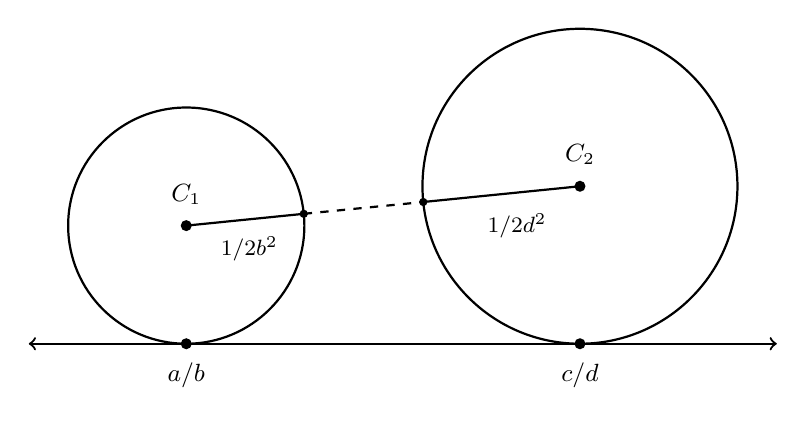
\begin{tikzpicture}[scale=2]
    \draw[thick](1,1) circle (1);
    \fill (1,1) circle (1pt);
    \fill (0.005,0.9) circle (0.75pt);
    \draw[thick](-1.5,0.75) circle (0.75);
    \fill (-1.5,0.75) circle (1pt);
    \fill (-0.7537,0.825) circle (0.75pt);
    \draw[<->,thick] (-2.5,0)--(2.25,0);
    \draw[dashed,thick] (-0.7537,0.825)--(0.005,0.9);
    \draw[thick] (0.005,0.9)--(1,1);
    \draw[thick] (-1.5,0.75)--(-0.7537,0.825);
    \foreach \x in {1,-1.5}
    {
    \fill (\x,0) circle (1pt);
    }
    \node[] at (1,-0.2) {\small $c/d$};
    \node[] at (-1.5,-0.2) {\small $a/b$};
    \node[] at (1,1.2) {\small $C_2$};
    \node[] at (-1.5,0.95) {\small $C_1$};
    \node[] at (-1.1,0.6) {\footnotesize $1/2b^2$};
    \node[] at (0.6,0.75) {\footnotesize $1/2d^2$};
\end{tikzpicture}\]
where $C_1$ and $C_2$ are the centres of the Ford circles atop $a/b$ and $c/d$ respectively.
\begin{align*}
\text{Cartesian coordinates of } C_1 &= \left(\dfrac{a}{b},\dfrac{1}{2b^2}\right)\\[0.5em]
\text{Similarly, cartesian coordinates of } C_2 &= \left(\dfrac{c}{d},\dfrac{1}{2d^2}\right)
\end{align*}
By Pythagoras' theorem (equivalently the distance formula)
\begin{align*}\label{smthng}
\overline{C_1C_2}^2 &= \left(\frac{1}{2b^2} - \frac{1}{2d^2}\right)^2 + \left(\frac{a}{b} - \frac{c}{d}\right)^2\\[0.5em]
&= \left(\frac{ad-bc}{bd}\right)^2 + \left(\frac{1}{2b^2} - \frac{1}{2d^2}\right)^2\tag{1}
\end{align*}
The Ford circles are tangent to each other if and only if
\begin{align*}
\overline{C_1C_2} &= \frac{1}{2b^2} + \frac{1}{2d^2}\\[0.5em]
\iff\overline{C_1C_2}^2 &= \left(\frac{1}{2b^2} + \frac{1}{2d^2}\right)^2\\[0.5em]
\underset{\refp{smthng}}{\iff}\left(\frac{ad-bc}{bd}\right)^2 + \left(\frac{1}{2b^2} - \frac{1}{2d^2}\right)^2 &= \left(\frac{1}{2b^2} + \frac{1}{2d^2}\right)^2\\[0.5em]
\iff\left(\frac{ad-bc}{bd}\right)^2 &= \left(\frac{1}{2b^2} + \frac{1}{2d^2}\right)^2 - \left(\frac{1}{2b^2} - \frac{1}{2d^2}\right)^2\\[0.5em]
\iff\left(\frac{ad-bc}{bd}\right)^2 &= 4\left(\frac{1}{2b^2}\right)\left(\frac{1}{2d^2}\right)\\[0.5em]
\iff(ad-bc)^2&= 1\\[0.5em]
\iff ad-bc&= \pm 1
\end{align*}
if and only if $\dfrac{a}{b}\kiss \dfrac{c}{d}$.
\end{proof}

\vspace*{1em}

\begin{proposition}\label{medsand}
Let $a/b$ be a reduced fraction. Then 
\begin{itemize}
\item[(1)] $a/b$ kisses infinitely many fractions.
\item[(2)] If $b>1$, then there are exactly two reduced fractions $c/d$ and $c'/d'$, with $d,d'<b$, that kiss $a/b$ such that $c/d \vee c'/d' = a/b$ and $c/d\kiss c'/d'$. 
\end{itemize}
\end{proposition}
\begin{proof}
\hfill
\begin{itemize}
\item[(1)] By assumption, $\gcd(a,b) = 1$. So, if $u/v$ is a reduced fraction kissing $a/b$, then by definition, $(x,y) = (v,u)$ is a solution to the equation
\[ax - by = \pm 1\]
We can take, without loss of generality, the equation $ax - by = 1$. Since $\gcd(a,b) = 1 = ax + (-b)y$, by Theorem \ref{ldea}, all solutions to this equation are of the form
\[u_n = u_0 + an,\quad v_n = v_0 + bn\qquad \text{(since $\lcm(a,-b) = -ab$)}\]
for any $n\in \zz$, where $(u_0,v_0)$ is a particular solution we obtain using the division algorithm.\\[1em]
There's at most one $n$ such that $v_n = 0$ since $b>0$. Whenever $v_n \neq 0$, $u_n/v_n$ or $-u_n/-v_n$ is a reduced fraction that kisses $a/b$.\\[1em]
Hence, there are infinitely many $u/v$'s that kiss $a/b$.\qed
\item[(2)] We have $b > 1$; let's plot the values of $\set{v_0 + bn}_{n \in \zz}$, say
\[\begin{tikzpicture}[scale=1.5]
    \draw[<->,thick] (-4,0)--(4,0);
	\foreach \x in {-3,-2,-1,0,1,2,3}
    {
    \fill (\x,0) circle (1.5pt);
    }
    \foreach \y in {3.3,2.3,1.3,0.3,-0.7,-1.7,-2.7}
    {
    \fill[color=indigo] (\y,0) circle (1pt);
    }
    \node[] at (0,-0.35) {$0$};
    \node[] at (1,-0.35) {$b$};
    \node[] at (2,-0.35) {$2b$};
    \node[] at (3,-0.35) {$3b$};
    \node[] at (-1.15,-0.35) {$-b$};
    \node[] at (-2.15,-0.35) {$-2b$};
    \node[] at (-3.15,-0.35) {$-3b$};
    \node[] at (4.5,0.5) {$b\zz$};
    \node[color=indigo] at (2.3,0.25) {\footnotesize $v_0$};
    \node[color=indigo] at (3.3,0.25) {\footnotesize $v_0 + b$};
    \node[color=indigo] at (1.3,0.25) {\footnotesize $v_0-b$};
    \node[color=indigo] at (0.3,0.25) {\footnotesize $v_0-2b$};
    \node[color=indigo] at (-0.7,0.25) {\footnotesize $v_0-3b$};
    \node[color=indigo] at (-1.7,0.25) {\footnotesize $v_0-4b$};
    \node[color=indigo] at (-2.7,0.25) {\footnotesize $v_0-5b$};
\end{tikzpicture}\]
Where could $v_0$ lie? We cannot have $v_0 = nb$ for any $n \in \zz$, since the fact $av_0 - bu_0 = 1$ gives us $b = (an - u_0) = a(nb) - bu_0 = 1$, that is, $b\mid 1$. This is isn't possible as $b > 1$. Hence $v_0 \in (kb,(k+1)b)$ for some integer $k$.\\
\\
Therefore, among $\set{v_0 + bn}_{n \in \zz}$, \emph{exactly one} falls in $(0,b)$ and \emph{exactly one} falls in $(-b,0)$. Let $v_m \in \set{v_0 + bn}_{n \in \zz}$ be the one in $(0,b)$; we can then also consider $u_m$.\\
\\
Then $u_m/v_m \kiss a/b$ and $0<v_m<b$, so define $c/d \coloneqq u_m/v_m$. Furthermore, also define $c'/d' \coloneqq (a - u_m)/(b-v_m)$, then $d' < b$ and
\[\frac{c}{d} \vee \frac{c'}{d'} = \frac{c+c'}{d+d'} = \frac{a}{b}\]
by constriction. Lastly, note that
\begin{align*}
cd' - c'd &= u_m(b-v_m) - (a-u_m)v_m\\[0.5em]
&= (bu_m - av_m) + (u_mv_m - u_mv_m)\\[0.5em]
&= -1
\end{align*}
Thus, $c/d \kiss c'/d'$.\qed
\end{itemize}\renewcommand{\qedsymbol}{}
\vspace*{-\baselineskip}
\end{proof}

\vspace*{1em}

\begin{corollary}[geometric form]
Let $a/b$ be a reduced fraction. Then
\begin{itemize}
\item[(1)] The Ford circle atop $a/b$ has infinitely many Ford circles tangent to it.
\[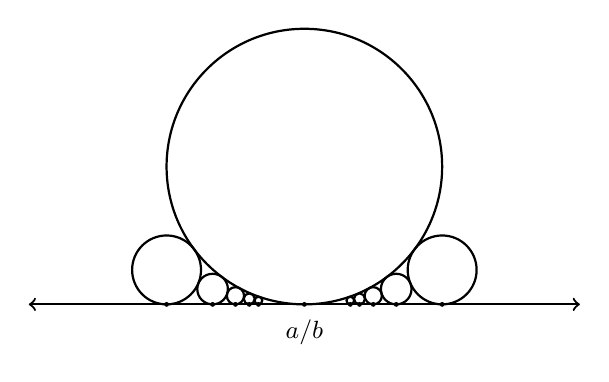
\begin{tikzpicture}[scale=3.5]
    \draw[thick](-2,0.5) circle (0.5);
    \draw[thick](-1.5,0.125) circle (0.125);
    \draw[thick](-1.66666,0.0555) circle (0.0555);
    \draw[thick](-1.75,0.03125) circle (0.03125);
    \draw[thick](-1.8,0.02) circle (0.02);
    \draw[thick](-1.8333,0.013889) circle (0.013889);
    \draw[thick](-2.5,0.125) circle (0.125);
    \draw[thick](-2.333,0.0555) circle (0.0555);
    \draw[thick](-2.25,0.03125) circle (0.03125);
    \draw[thick](-2.2,0.02) circle (0.02);
    \draw[thick](-2.1666,0.013889) circle (0.013889);
    \draw[<->,thick] (-3,0)--(-1,0);
    \foreach \x in {-2,-1.5,-1.66666,-1.75,-1.8,-1.8333,-2.5,-2.333,-2.25,-2.2,-2.1666}
    {
    \fill (\x,0) circle (0.25pt);
    }
    \node[] at (-2,-0.1) {\small $a/b$};
\end{tikzpicture}\]
\item[(2)] If $b>1$, then among the infinitely many Ford circles as above, there are exactly two whose mediant is the Ford circle atop $a/b$.
\[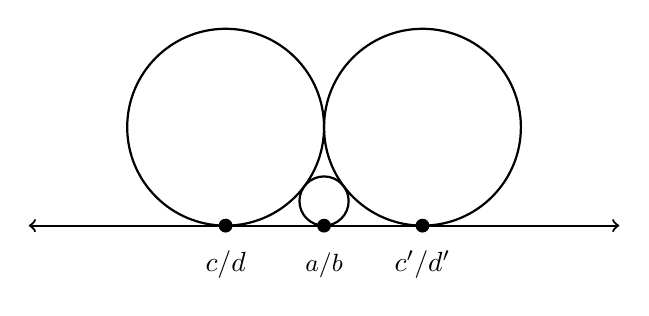
\begin{tikzpicture}[scale=2.5]
    \draw[thick](-2,0.5) circle (0.5);
    \draw[thick](-1,0.5) circle (0.5);
    \draw[thick](-1.5,0.125) circle (0.125);
    \draw[<->,thick] (-3,0)--(0,0);
    \foreach \x in {-2,-1,-1.5}
    {
    \fill (\x,0) circle (1pt);
    }
    \node[] at (-1,-0.2) {$c'/d'$};
    \node[] at (-2,-0.2) {$c/d$};
    \node[] at (-1.5,-0.2) {\small $a/b$};
\end{tikzpicture}\]
\end{itemize}
\end{corollary}

\vspace*{1em}

\begin{example}
Find the two kissing (reduced) fractions whose mediant is $83/71$.
\end{example}
\begin{proof}[Answer]
If $x/y$ was one of them, then $71x - 83y = \pm 1$. Let's employ the division algorithm
\begin{align*}
83 &= 71(1) + 12\\[0.5em]
71 &= 12(5) + 11\\[0.5em]
12 &= 11(1) + 1\\[0.5em]
11 &= 1(11) + 0
\end{align*}
Running this backwards, we get $1 = 71 (-7) + 83 (6)$ and so $-1 = 71(7) - 83(6)$.\\
\\
Take $\dfrac{c}{d} = \dfrac{7}{6}$, note $6 < 71$, and $\dfrac{c'}{d'} = \dfrac{83-7}{71-6} = \dfrac{76}{65}$.
\end{proof}

\vspace*{1em}

\begin{example}[in-class]
Find the two kissing (reduced) fractions $a/b$ and $c/d$ whose mediant is $15/32$.
\end{example}

\vspace*{1em}

\begin{theorem}
Consider the following process
\begin{itemize}
\item \emph{Step I.} Start with fractions $\dfrac{n}{1}$ as $n$ runs through the integers.
\item \emph{Step II.} Whenever you see two kissing fractions, form their mediant.
\item \emph{Step III.} Keep repeating \emph{Step II}.
\end{itemize}
Then
\begin{itemize}
\item[(1)] The fractions occurring in this sequence are reduced.
\item[(2)] Conversely, all reduced fractions occur in this sequence.
\end{itemize}
\end{theorem}
\begin{proof}
We induct on the the denominator of $a/b$, where $a/b$ is an element of the sequence.
\begin{itemize}
\item[(1)] For $b = 1$, $a/1$ is reduced.\\[0.5em]
Assume the inductive hypothesis; if $\dfrac{a}{b}\kiss \dfrac{c}{d}$, we form $\dfrac{a}{b}\vee \dfrac{c}{d} = \dfrac{a+c}{b+d}$.
\vspace*{0.2in}
\begin{subproof}
\vspace*{-0.1in}
\begin{lemma}\label{medkiss}
Suppose $\dfrac{x}{y} \kiss \dfrac{z}{w}$, then $\left(\dfrac{x}{y}\vee \dfrac{z}{w}\right)\kiss \dfrac{x}{y},\dfrac{z}{w}$.
\end{lemma}
\begin{proof}
We verify directly; since $x/y \kiss z/w$, i.e. $xy - yz = \pm 1$, note that
\begin{align*}
w(x+z) - z(y+w) &= xw + wz - yz - wz\\[0.5em]
&= xw - yz = \pm 1
\end{align*}
Therefore $\dfrac{x}{y}\vee \dfrac{z}{w} = \dfrac{x+z}{y+z} \kiss \dfrac{z}{w}$; similarly $\left(\dfrac{x}{y}\vee \dfrac{z}{w}\right) \kiss \dfrac{x}{y}$.
\end{proof}
\end{subproof}
%\vspace*{0.2in}
Now, since $\left(\dfrac{a}{b}\vee \dfrac{c}{d}\right) \kiss \dfrac{a}{b}$, the mediant is reduced by Proposition \ref{redkiss}.\qed

\item[(2)] If $b = 1$, then $\dfrac{a}{1}$ occurs in the base step.\\
\\
Assume the inductive hypothesis; now $b > 1$, therefore by Proposition \ref{medsand} there exist reduced fractions $c/d$ and $c'/d'$ with $d,d' < b$ such that 
\[\dfrac{c}{d} \vee \dfrac{c'}{d'} = \dfrac{a}{b}\]
$c/d$ and $c'/d'$ occur in the sequence by the inductive hypothesis. Therefore, so does $a/b$ as their mediant.\qed
\end{itemize}\renewcommand{\qedsymbol}{}
\vspace*{-\baselineskip}
\end{proof}

\vspace*{1em}

\begin{theorem}[Dirichlet's Approximation Theorem]
Let $x$ be an irrational real number. Then there exist infinitely many reduced fractions $a/b$ such that
\[\abs{x- \frac{a}{b}} < \frac{1}{2b^2}\]
\end{theorem}
\begin{proof}
\emph{I.} Start with $b=1$, $x$ is in the shadow of exactly Ford circle atop $\dfrac{a}{1}$
\[\begin{tikzpicture}[scale=2.5]
    \draw[thick](-2,0.5) circle (0.5);
    \draw [draw=none, fill=lightgrey] (-1.5,-0.1) rectangle (-1,0.5);
    \draw[thick,black,fill=white](-1,0.5) circle (0.5);
    \draw[<->,thick] (-3,0)--(0,0);
    \foreach \x in {-2,-1}
    {
    \fill (\x,0) circle (1pt);
    }
    \node[] at (-1,-0.2) {$a$};
    \node[] at (-2,-0.2) {$a-1$};
    \fill[color=indigo] (-1.3,0) circle (1pt);
    \node[color=indigo] at (-1.3,-0.2) {$x$};
\end{tikzpicture}\]
But then
\[\abs{x - \frac{a}{1}} < \frac{1}{2}\]
\vspace*{0.5em}\\
\emph{II.} Consider a Ford circle atop $a/b$ which shadows $x$.
\[\begin{tikzpicture}[scale=4]
%    \draw[thick](-2,0.5) circle (0.5);
    \draw [draw=none, fill=lightgrey] (-1.5,-0.035) rectangle (-2.5,0.45);
    \draw[thick,black,fill=white] (-1.5,0.5) (-2.5,0.5) arc(0:180:-0.5);
    \draw[<->,thick] (-3,0)--(-1,0);
    \fill (-2,0) circle (0.5pt);
    \node[] at (-2,-0.1) {\small $a/b$};
    \fill[color=indigo] (-1.7,0) circle (0.5pt);
    \node[color=indigo] at (-1.7,-0.1) {$x$};
\end{tikzpicture}\]
Since $x$ is an irrational real number, so either $x>a/b$ or $x< a/b$. Let's treat the case $x > a/b$.\\
\begin{subproof}
{\bf Claim.} \emph{There exists a reduced fraction $\dfrac{c}{d}>\dfrac{a}{b}$ such that $d\leq b$ and $\dfrac{c}{d}\kiss \dfrac{a}{b}$}
\begin{proof}[Proof of Claim]
If $b = 1$, take $\dfrac{c}{d} = \dfrac{a+1}{1}$.\\
\\
If $b>1$, then by Proposition \ref{medsand} we can find reduced fractions $x/y$ and $x'/y'$ with $y,y'<b$ such that $a/b$ is their mediant. Let $c/d$ be one of these fractions that lies to the right of $a/b$ and by Lemma \ref{medkiss} we know that $c/d \kiss a/b$.
\end{proof}
\vspace*{0.005em}
\end{subproof}
\vspace*{0.5em}
\begin{minipage}{0.4\textwidth}
Consider the chain
\vspace*{0.3em}
\begin{align*}
\frac{a}{b} \vee \frac{c}{d} &= \frac{e}{f}\\[0.5em]
\frac{a}{b} \vee \frac{e}{f} &= \frac{g}{h}\\[0.1em]
\quad\vdots
\end{align*}
\end{minipage}
\begin{minipage}{0.6\textwidth}
\[\begin{tikzpicture}[scale=3.3]
    \draw[thick](-2,0.5) circle (0.5);
    \draw[thick](-1,0.5) circle (0.5);
    \draw[thick](-1.5,0.125) circle (0.125);
    \draw[thick](-1.66666,0.0555) circle (0.0555);
%    \draw[thick](-1.75,0.03125) circle (0.03125);
%    \draw[thick](-1.8,0.02) circle (0.02);
%    \draw[thick](-1.8333,0.013889) circle (0.013889);
    \draw[<->,thick] (-2.5,0)--(-0.5,0);
%    \foreach \x in {-2,-1.5,-1.66666,-1.75,-1.8,-1.8333}
    \foreach \x in {-2,-1.5,-1.66666,-1}
    {
    \fill (\x,0) circle (0.5pt);
    }
    \node[] at (-2,-0.15) {\footnotesize $\dfrac{a}{b}$};
    \node[] at (-1,-0.15) {\footnotesize $\dfrac{c}{d}$};
    \node[] at (-1.5,-0.15) {\footnotesize $\dfrac{e}{f}$};
    \node[] at (-1.66666,-0.15) {\footnotesize $\dfrac{g}{h}$};
    \node[] at (-1.825,-0.15) {\footnotesize $\cdots$};
\end{tikzpicture}\]
\end{minipage}
\vspace*{0.5em}\\
The shadows of all these Ford circles cover the right shadow under $a/b$. So, at least one of the Ford circles in the chain must shadow $x$. Let's call the rational number this Ford circle is atop $a_1/b_1$, where $b_1 < b$.
\[\begin{tikzpicture}[scale=2.5]
    \draw [draw=none, fill=lightgrey] (-1.5,-0.05) rectangle (-1,0.5);
    \draw[thick,black,fill=white](-1,0.5) circle (0.5);
    \draw[<->,thick] (-2,0)--(0,0);
    \foreach \x in {-1}
    {
    \fill (\x,0) circle (1pt);
    }
    \node[] at (-1,-0.25) {\small $\dfrac{a_1}{b_1}$};
    \fill[color=indigo] (-1.3,0) circle (1pt);
    \node[color=indigo] at (-1.3,-0.17) {$x$};
\end{tikzpicture}\]
The radius of the circle $=\dfrac{1}{2}(\text{diameter}) = \dfrac{1}{2b_1^2}$. So,
\[\abs{x - \frac{a_1}{b_1}}<\frac{1}{2b_1^2}\]
The case $x< a/b$ is similar (everything happens on the left). The theorem follows by starting with \emph{I.} and repeatedly applying \emph{II.}
\end{proof}

\vspace*{1em}

\begin{remark}[Warning/Clarification]
The theorem doesn't imply that this approximation works for \emph{every} integer $b$.\\[0.5em]
\emph{e.g.}\quad $\pi = 3.1415926\ldots$\\[0.5em]
For $b = 1$, we have $\abs{\pi - 3} < \dfrac{1}{2}$.\\[1em]
For $b = 2$, we cannot find an $\dfrac{a}{2}$ such that \[\abs{\pi - \dfrac{a}{2}}<\dfrac{1}{2\cdot 2^2}.\] Because the smallest fraction of this form is $\dfrac{7}{2} = 3.5$ and $\abs{\pi - 3.5} \approx 0.36$ while $\dfrac{1}{2\cdot 2^2} = 0.125$.\\[1em]
But $b = 7$ works, take $\dfrac{a}{b} = \dfrac{22}{7}$.
\end{remark}

%\vspace*{0.5in}

\subsection{Problems}
\vspace{0.1in}

\begin{problem}\label{Problem 7.1}
Write a formula which describes all fractions that kiss $7/11$.
\end{problem}